\section{Introduction}
The register-transfer level (RTL) programming model paved the road for Verilog and VHDL to flourish as the leading hardware description languages (HDLs) in the electronic design automation industry. However, that road is steadily nearing its end, as both hardware designs and devices become increasingly more complex. While the software world is striving for a "write once, run anywhere" programmability, an RTL design with the same requirements may vary greatly across different FPGA and ASIC devices that incorporate various technologies and core components. Moreover, minor requirement changes may lead to significant design changes, since RTL abstraction prevents separation of functionality and timing constraints. For example, registers serve various roles such as preserving a state, pipelining and balancing a data path, deriving timed signals from an input clock, and synchronizing an input signal. This coupling between core requirements and device constraints leads to verbose and unportable RTL designs. 

Ongoing efforts to bridge this hardware programmability gap~\cite{Kapre2016, Nane2016, Windh2015} can be split into two major tracks: high-level synthesis (HLS) tools and high-level RTL (HL-RTL) languages.
On the one hand, HLS tools (such as Vivado~\cite{Vivado2012}, Catapult~\cite{graphics2008catapult}, and others~\cite{Kavvadias2013, synphony2015}) rely on modern programming languages like C or M and apply  auto-pipelining and optimization mechanisms to make hardware accelerators accessible to non-hardware engineers. While this approach has proven successful in algorithmic acceleration domains, such languages carry von Neumann sequential semantics and thus hinder construction of parallel hardware, which is required to describe architectures~\cite{Zhao2017}. Even a simple periodic led toggle is impossible to generate via HLS languages.
On the other hand, HL-RTL languages (such as Chisel~\cite{Bachrach2012}, Bluespec~\cite{nikhil2004bluespec}, PyRTL~\cite{Clow2017}, and others~\cite{Charles2016, Liu2017, jiang2018mamba, decaluwe2004myhdl, CxLang2014, Lockhart2014}) try to enhance productivity by introducing new hardware generation constructs and semantics but without abstracting over register-level description (even Bluespec that uses concurrent guarded atomic actions assumes rules complete within a single clock cycle). Therefore, HL-RTL designs still suffer under the \emph{"tyranny of the clock"}~\cite{Sutherland2012} and are bound to specific timing and target constraints.


In this paper we further extend DFiant~\cite{Port2017}, a modern HDL whose goal is to improve hardware programmability and designer productivity by enabling designers to express truely portable and composable hardware designs.
DFiant decouples functionality from timing constraints (in an effort to end the \emph{"tyranny of the clock"}~\cite{Sutherland2012}). DFiant offers a clean model for hardware construction based on its core characteristics:
\begin{enumerate*}[label=(\roman*)]
\item
  a clock-agnostic dataflow model that enables implicit parallel data and computation scheduling; and
\item
  functional register/state constructs accompanied by an automatic pipelining process, which eliminate all explicit register placements along with their direct clock dependency.
\end{enumerate*} DFiant borrows and combines constructs and semantics from software, hardware and dataflow languages. Consequently, the DFiant programming model accommodates a middle-ground approach between low-level hardware description and high-level sequential programming. 

\begin{figure*}[t]
	\centering
	\captionsetup{justification=centering}
	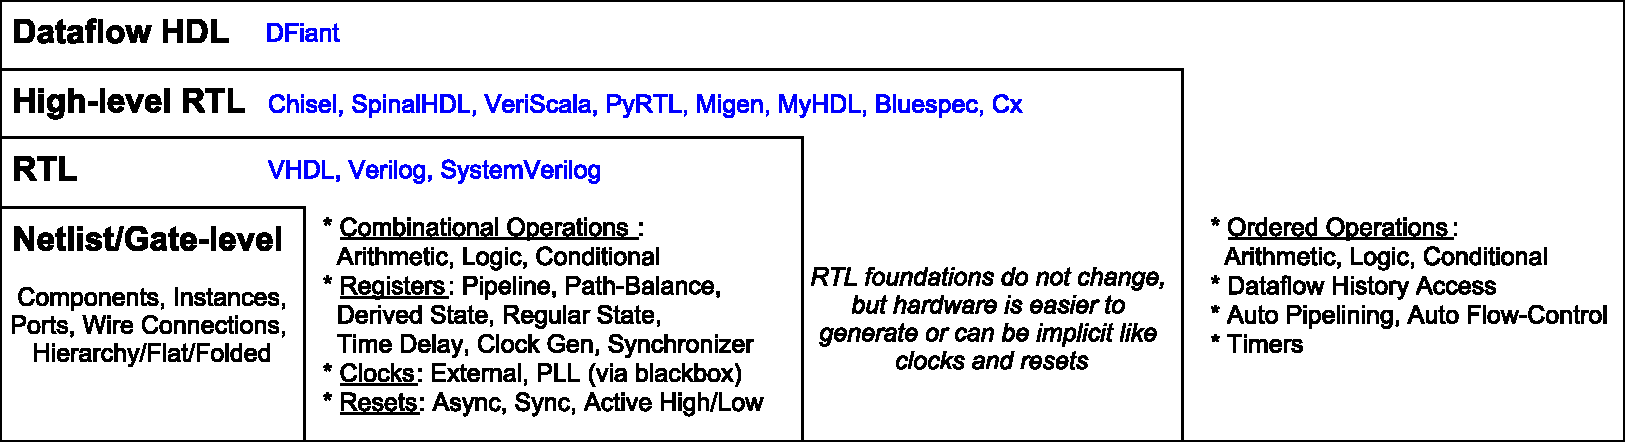
\includegraphics[width=\linewidth]{graphics/motivation.pdf} 
	\captionof{figure}{HDL abstraction layer summary (lowest=netlist, highest=dataflow) \\ DFiant is the first language to support the highest layer, a dataflow HDL.}
	\label{fig:motivation}
\end{figure*}

%\newpage %equivalent to when author names aren't removed
DFiant is implemented as a Scala library and relies on Scala's strong, extensible, and polymorphic type system to provide its own hardware-focused type system (e.g., bit-accurate dataflow types, input/output port types). The library performs two main tasks: the frontend compilation, which translates dataflow variable interactions into a dependency graph; and the backend compilation, which translates the graph into a pipelined RTL code and a TCL constraints file, followed by a hardware synthesis process using commercial tools. Additionally, the graph can be simulated within the Scala integrated development environment (IDE). 

This work focuses on the DFiant language and frontend compiler. DFiant is \emph{not} an RTL language, nor is it a sequential language such as C. The following two sections highlight DFiant's unique semantics by comparing them against modern design language alternatives. For a proof of concept, we implemented a preliminary auto-pipelining backend compiler to compare DFiant and traditional HDL design flows in two test cases: an Advanced Encryption Standard~\cite{pub2001197} (AES) cipher block and an IEEE-754~\cite{IEEE2008} floating point multiplier (FPMul). Future work may delve further into the backend compiler and its HLS potential.


The paper is organized as follows. The next section describes the motivation for the dataflow HDL abstraction layer, followed by Section~\ref{sec:dfiant}, which provides a general overview of the DFiant HDL language. 
Section~\ref{sec:evaluation} provides results, and finally, Section~\ref{sec:conclusion} concludes the paper.




%\newpage
%Interactions between DFiant types lead to hardware construction, while non-DFiant types (e.g. Integer) are considered as constants. 
 

%Modern designs are rich with arithmetic functionality. Surely the designer cannot explicitly pipeline everything manually and must be selective. On one hand, under-pipelining may lead to insufficient performance and redesign iterations. On the other hand, over-pipelining might lead to performance reduction due to limited room for logic and routing, in addition to wasting design time, energy, and device resources. 

%Typical FPGA devices now include clock generators, serializers, PCI express cores, internal memory blocks, external memory interfaces, and many other proprietary modules. Evidently, formulating designs that are transportable across devices and timing variance is difficult, if not impossible. Complex logic design has become a task fit only for experts. 
% The generic code annotations enabling this are cumbersome and limited. 



